\documentclass{sigchi}

% Use this command to override the default ACM copyright statement (e.g. for preprints). 
% Consult the conference website for the camera-ready copyright statement.


%% EXAMPLE BEGIN -- HOW TO OVERRIDE THE DEFAULT COPYRIGHT STRIP -- (July 22, 2013 - Paul Baumann)
% \toappear{Permission to make digital or hard copies of all or part of this work for personal or classroom use is 	granted without fee provided that copies are not made or distributed for profit or commercial advantage and that copies bear this notice and the full citation on the first page. Copyrights for components of this work owned by others than ACM must be honored. Abstracting with credit is permitted. To copy otherwise, or republish, to post on servers or to redistribute to lists, requires prior specific permission and/or a fee. Request permissions from permissions@acm.org. \\
% {\emph{CHI'14}}, April 26--May 1, 2014, Toronto, Canada. \\
% Copyright \copyright~2014 ACM ISBN/14/04...\$15.00. \\
% DOI string from ACM form confirmation}
%% EXAMPLE END -- HOW TO OVERRIDE THE DEFAULT COPYRIGHT STRIP -- (July 22, 2013 - Paul Baumann)


% Arabic page numbers for submission. 
% Remove this line to eliminate page numbers for the camera ready copy
 \pagenumbering{arabic}


% Load basic packages
%\usepackage{biblatex}
\usepackage{balance}  % to better equalize the last page
\usepackage{graphics} % for EPS, load graphicx instead
\usepackage{times}    % comment if you want LaTeX's default font
\usepackage{url}      % llt: nicely formatted URLs
\usepackage{listings}
\usepackage[T1]{fontenc}
\usepackage[utf8]{inputenc}
\usepackage{microtype}
\usepackage{subcaption}

\lstset{basicstyle=\footnotesize\ttfamily,breaklines=true}
% llt: Define a global style for URLs, rather that the default one
\makeatletter
\def\url@leostyle{%
  \@ifundefined{selectfont}{\def\UrlFont{\sf}}{\def\UrlFont{\small\bf\ttfamily}}}
\makeatother
\urlstyle{leo}


% To make various LaTeX processors do the right thing with page size.
\def\pprw{8.5in}
\def\pprh{11in}
\special{papersize=\pprw,\pprh}
\setlength{\paperwidth}{\pprw}
\setlength{\paperheight}{\pprh}
\setlength{\pdfpagewidth}{\pprw}
\setlength{\pdfpageheight}{\pprh}

% Make sure hyperref comes last of your loaded packages, 
% to give it a fighting chance of not being over-written, 
% since its job is to redefine many LaTeX commands.
\usepackage[pdftex]{hyperref}
\hypersetup{
pdftitle={Graphical Structured Temporal Programming for Interactive Applications},
pdfauthor={Jean-Michaël Celerier},
pdfkeywords={SIGCHI, proceedings, archival format},
bookmarksnumbered,
pdfstartview={FitH},
colorlinks,
citecolor=black,
filecolor=black,
linkcolor=black,
urlcolor=black,
breaklinks=true,
}

% create a shortcut to typeset table headings
\newcommand\tabhead[1]{\small\textbf{#1}}


% End of preamble. Here it comes the document.
\begin{document}

\title{Graphical Structured Temporal Programming for Interactive Applications}

\numberofauthors{3}
\author{
  \alignauthor Redacted\\
    \affaddr{Redacted}\\
    \affaddr{Redacted}\\
    \email{Redacted}
  \alignauthor Redacted\\
    \affaddr{Redacted}\\
    \affaddr{Redacted}\\
    \email{Redacted}    
  \alignauthor Redacted\\
    \affaddr{Redacted}\\
    \affaddr{Redacted}\\
    \email{Redacted}
}

\maketitle

\begin{abstract}
  The development of interactive shows and interactive user interfaces for arts \& exhibitions
has traditionally been done with tools that pertain to two broad metaphors. 
Cue-based environments work by making groups of parameters and sending them to remote devices, 
while more interactive applications are generally written in domain-specific 
programming environments, like Max/MSP, Processing or OpenFrameworks.
  In this paper, we argue about the specific issues that arise in such environments, and we present 
i-score : an extensive and collaborative software suite that bridges
the gap between time-based, logic-based and flow-based interactive application authoring tools. 
This is done in a single cohesive graphical user interface, built upon a few simple and novel primitives.
  i-score allows the creation of software meant for operation in a large parameter space, 
and enables artists to express easily both temporal logic and structured programming, 
with facilities for automating and applying transformations to single and multi-dimensional parameters.
\end{abstract}

%\keywords{
%	Guides; instructions; author's kit; conference publications;
%	keywords should be separated by a semi-colon. \newline
%	\textcolor{red}{Optional section to be included in your final version, 
%  but strongly encouraged.}
%}

\category{D.2.2}{Design Tools and Techniques}{User interfaces}

%See: \url{http://www.acm.org/about/class/1998/}
%for more information and the full list of ACM classifiers
%and descriptors. \newline
%\textcolor{red}{Optional section to be included in your final version, 
%but strongly encouraged. On the submission page only the classifiers’ 
%letter-number combination will need to be entered.}

\section{Introduction}
This paper presents a paradigm that aims to allow non-programmers 
to conceive interactive applications easily and execute them in production. These interactive applications can be either musical pieces, interactive shows where the interaction may come from the performer, or even the spectators, museum installations and graphical interfaces.

The existing software stack is either oriented too much towards the 
cue paradigm, which is useful as long as there is no complex logic involved, 
or towards the programming paradigm, where it is hard to write simple scenarios 
like "move a spotlight in horizontal oscillation for ten seconds; after the first 5 
seconds, if a dancer jumps on the stage, then play a sound and increase reverberation steadily as long as the dancer is on stage".

We will first present the current practices on the field, including the depiction of three specific artistic installations revolving around the idea of a computer-controlled orchestration.

We will then explain the paradigm of the i-score software suite, which allows to express complex scenarios in a single graphical interface. These scenarios involve both temporal logic and structured programming. They can afterwards be deported or even embedded in other tools thanks to a C++ API. 

Our constructs will be presented by starting with the purely temporal ones, 
and then by extend to the elements relevant in a structured programming context.
Finally we will see how data is handled throughout the software.

This model has evolved through many stages of refinement, first starting as an application of 
Allen's relationships\cite{allen1983maintaining} and moving on to concurrent constraint models\cite{allombert2006concurrent,toro2010concurrent}, Petri nets\cite{allombert2007system,arias2014modelling}, finite automatons\cite{arias2015exploiting}, and reactive languages\cite{ariasexecuting}, which are all formal approaches which have each their advantages and drawbacks. 

These different formal models are compared in~\cite{celerier2015ossia}, along with a more thorough presentation of the execution semantics of the present model.

The present document takes the point of view of an user that would approach the graphical user interface. However, most of the concepts are actually implemented in a C++ API\cite{hogue2014ossia} that can be used to generate scenarios directly from code. Moreover, some concepts in the graphical interface are themselves built upon primitives offered in the API.

\subsection{Motivation}
The need for authoring software able to operate in both the temporal and logical domains arises as soon as an artist wants to set-up a show which may have different outcomes according to the actions of the performer, or even of the participants.

\subsection{Use cases}
To explain properly the kind of artistic demeanors we are working with, three case studies will follow : two musical pieces and a museum installation. Another target for the method that we propose is the development of interactive kiosk-like user interfaces.

\paragraph{Klavierstück XI}
This is a music piece composed in 1957 by Karlheinz Stockhausen.

The interpretation plays a huge part on the piece. It is composed of multiple "segments", a bit longer than musical bars. This is called a polyvalent structure.

The performer starts with one of the segments. When he finishes playing a segment, he chooses another randomly. When he wants to choose a segment that he has already played two times, the music stop.

The number of possible combinations is so high that any given interpretation made by chosing the segments randomly would likely be played for the first time.

This can be modelled easily by maintaining counters for each segment, incrementing the counter when it is played, and having a global loop whose looping condition is \texttt{no counter is greater than 2}. However the musical parts would have to be written in a specific music-sheet oriented software.

\paragraph{Pianotronics \#3}
Alain Bonardi is a french electro-acoustic composer; in this musical piece there are ten blocks that each contain a small part of piano sheet music; an external algorithm does a random draw of these blocks. There are some similarities with Stockhausen's piece, but, instead of leaving the choice of the order to the performer, it's the algorithm that makes the choice and the performer has to interpret the sheet music that is being shown to him in real time. In addition, each block contains controls for background music to play in ambisonics, independently of what the pianist is doing.

Since a computer is generating the sheet music, the performer has to follow everything quickly. However, the interpretation can have a small degree of freedom : the performer's playing is recorded and compared with the displayed sheet music. When an algorithm detects that the part was successfully played, or if a timeout has expired, it then moves on to the next part.

\paragraph{The Runner}
This is an actual museum installation that is located in the Futuroscope, at the city of Poitiers in France. The goal is for children to test their running speed and compare themselves against a leaderboard of the best runners that took the attraction. It is based around two movement detectors, one at the beginning and one at the end of the running lane. However, there is some complexity involved to prevent the children from cheating, for instance by having one of their friends trigger the "finish line" sensor just after they triggered the start sensor. Timeouts are also necessary if a participant starts running but decides to never finish, not triggering the end sensor.

Precisely, the installation can be explained as follows : 
\begin{itemize}
    \item A "welcome" loop that displays a looping video and waits for an interaction.
    \item A main running loop, that starts after the triggering of the start sensor. It begins with a fixed duration announce video that goes "3.. 2.. 1..". While the child runs, there is another video and some music playing. 
    \begin{itemize}
    	\item If the final sensor is triggered before 5 seconds, it is considered cheating and we break out of the main loop.
    	
    	\item Else, if the final sensor is not triggered after 30 seconds, the race is considered abandoned. 
    	
    	\item If the main loop does not end in one of these "erroring" states, there is a standard finish video that lasts 5 seconds and shows the position of the current run in the podium. After a few seconds, we return to the welcome loop.
    \end{itemize}
      
    
    \item Overarching all this, there is a topmost loop that regularly checks if the installation is correctly networked with the museum backend. If it's not the case, everything is stopped and a generic "Please call a technician" message is shown.
\end{itemize}

\begin{figure}
    \centering
    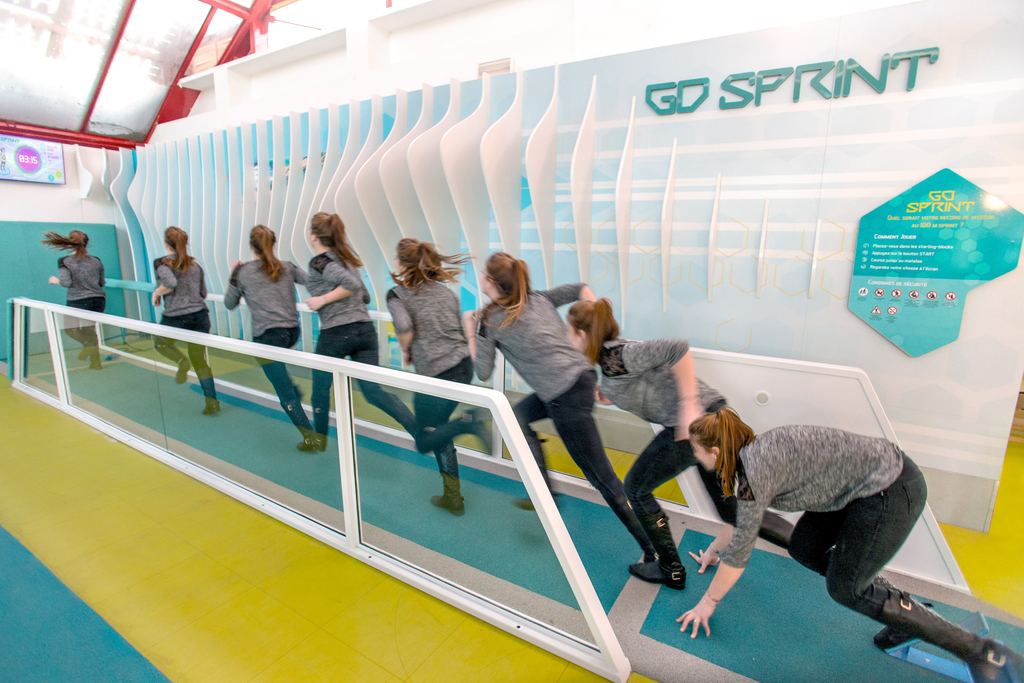
\includegraphics[scale=0.6]{images/futuroscope.jpg}
    \caption{The Runner installation. \tiny{©JL AUDY/FUTUROSCOPE}}
    \label{fig.futuroscope}
\end{figure}

Currently, the whole logic is implemented in Max/MSP. A picture can be seen in fig.~\ref{fig.futuroscope}.

% Dire que pour i-score il manque juste la possibilité de gérer des "sorties" à tout instant.

\subsection{Existing approaches}
Now that we have exposed the kind of problems that we are tackling, we are going to review the existing methods that have been and are still used to conceive and run interactive applications.

There are mostly three parts : first, the cue-based tools. This is a broad range which can go from extremely specialized software that would for instance only handle video, to more generic solutions that aim to control different kinds of media.

Then, the text-based programming tools. These are programming languages that are dedicated to the task of building interesting interactive applications and their user interfaces.

Finally, there are specific flow-control models; they are between both axes. i-score fits into this category.

In addition, we will have an overview of document object model paradigms. This is to present the kind of software that i-score is expected to control. % Peut-être mettre ça ailleurs, plus loin ?

\subsubsection{Cue-based environments}
This is the first kind of environment for content creation, and certainly one of the most used for shows, because it mimics the behaviour of real hardware such as lighting consoles.

A cue is a set of data that maps to a certain state on stage. For instance, there would be a cue for the beginning of a new scene in a pièce de théâtre, that would set the lights in the correct positions and colors, and start playing a background music.

In this kind of environment, there is no manifest temporal relationships to speak of: the cue are organized in stacks that will generally follow the expected development of the show. A human is generally present to trigger the correct cues at the correct time, and adjusts if something goes wrong on stage.

An example of cue-based system for show control is given by Kim Youngjae in~\cite{kim_unified_2013}. 

This is also similar to the session view of Ableton Live, with stacks of audio clips that are to be triggered by the performer. The timeline view of Live, however, does not enable interactivity. Modulo Pi is another hardware and software facility that works with video cues.

These environments, overall, allow to set-up a show very easily - sometimes dragging and dropping the desired cues will be enough. But as soon as there is interactivity involved, this paradigm becomes useless : there is absolutely no flexibility apart from the one provided by a human operator, which may become overwhelmed if too much things happen on stage at the same time.

\subsubsection{Programming-based environments}
At the other range of capabilities lies the full-blown programming languages. They allow complete flexibility over what's happenning. However, very few artists are eager to learn how to program in order to write interactive show; besides, when the show relies heavily on temporal elements, the textual structuration doesn't make the flow of the program easy to understand, as can be seen in fig.~\ref{fig.hardtofollow}.

\begin{figure}
\begin{lstlisting}[language=c++]
GlobalState state;

void light1()
{
  state["/light/r"] = 255;
  usleep(200000);    
  state["/light/r"] = 0;
  for(int i = 0; i < 100; i++)
  {
    if(state["/sound/volume"] > 50)
      state["/light/g"] = i;        
    state["/light/b"] = 255 - i;
    usleep(32000);
  }
}

void scenario()
{
  state["/sound"] = true;
  light1();
  usleep(10000);
  light1();
}
\end{lstlisting}
\caption{A trivial light-changing program. However, the lack of cohesion between the code's organization and the temporal behaviour makes the development of the scenario hard to visualize. Time, logic and data are highly coupled, which makes it even harder to follow.}
\label{fig.hardtofollow}
\end{figure}

The programmer also needs to keep track of the available data and devices that he can access; this is commonly achieved by using god objects that represent the external devices's state or something akin to Haskell's \texttt{RealWorld} concept\cite{launchbury1995state}. Else, a state-keeping object has to be passed across most of the method and function calls, which incurs a certain cost on the complexity of such software. Another common problematic is the method used to represent external devices. Some libraries will rather try to implement everything with the language's primitives and structures. Hence, an address of a device would be represented by a tree-like structure. Other would take an approach closer to a domain-specific language, by specifying the addresses in textual format that are to be parsed behind the scene. 

Besides, another problem is reusability : most of the interactive applications are to be used once and then discarded since they are most of the time very different. Libraries exist, but even then they are generally customized by the final application author. Hence, any system wishing to improve on the current state of affairs would have to provide easy-to-use library facilities.

Finally, the standard primitive for parallelization, threads, is highly unpractical to use because of the indeterminism of the operating system's scheduler. Other programming paradigms, like reactive programming, offers better tools to solve the problem of the control of multiple kinds of data at the same time; however it then becomes harder to have a scenario split into multiple, unrelated parts that would follow each other.

For instance, one can write such software with ActionScript (part of the Adobe Flash environment), Processing (a set of multimedia libraries based on Java) and OpenFrameworks, which is to C++ what Processing is to Java\cite{noble2009programming}. These languages or frameworks are general-purpose, but contain a lot of multimedia-oriented tools, to playback and modify video, or create particle systems. 

Some domains have more specific tools : for instance, the LISP community has produced a wealth of languages able to represent and produce non-interactive and interactive music, like CommonMusic\cite{taube1997introduction} or Nyquist\cite{dannenbergnyquist}. INscore\cite{fober2013programming} and Antescofo with Ascograph\cite{coffy2014ascograph} are two other softwares dedicated the composition and authoring of interactive music scores, both with a dedicated domain-specific language and a GUI to control it.

\subsubsection{Graphical programming interactive applications}
A lot of approaches exist with regards to visual programming. However, not all are conceived with the idea of managing time in mind. Those that are generally geared towards the kind of applications that we are interested in, or video games.

A first instance of simple graphical programming language is Scratch\cite{resnick2009scratch}, built at the MIT. The language is very close from standard structured programming, with explicit conditional and looping constructs; however building a program is done by assembling boxes together instead of typing.

Then, many environments are stemming from the data flow model. For instance, it is implemented in video game engines like Unreal Engine's Blueprint system\cite{shah2014mastering}. Data-flow programming is based on the computation of the result of an operation not when it is asked for by the programmer, like it is done with imperative programming, but when the operands of the operation are set. Hence, the programmer describes an invariant and values that come from external sensors (or generators) are pumped into the system and transformed in an output.
The most used in artistic and interactive installations are patcher software, like Max/MSP or PureData. Patchers use the data-flow model. A specific patcher software for audio algorithms exists : Integra Live\cite{bullock2011integra}.

Finally, not all flow programming languages are meant to produce real-time applications. For instance, OpenMusic\cite{bresson_openmusic:_2011} is a graphical language used for the generation of sheet music.

Generally, data-flow based programming language's graphical representation are graphs, where the nodes are computations and the directed edges move the output of a computation to the input of another.
But there are other forms of multimedia-oriented graphical languages that put the emphasis on the time instead of the computations in their graphs. For instance, applications build with the MEF++ frameworks\cite{ackermann_direct_1994} represents time in boxes that can contain arbitrary multimedia data. The question of variable time has also been tackled with constraint solving algorithms in \cite{song_interactive_1999}; although it is only useful during the authoring part : the execution of the created multimedia "programs" is fixed.

We will now present the model that has been built in order to be able to develop easily the kind of artistic installations that have been exhibited in the first part of this document. The methodology that has been used is domain driven design with contributions of a small commitee of experts and practicioners in the authoring of interactive installations. 
\section{Temporal structure}\label{sec.temporal}
\begin{figure}[h]
    \centering
    \begin{minipage}[b]{.5\linewidth}
        \centering
        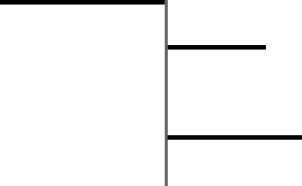
\includegraphics[scale=0.6]{images/timenode.png}
        \subcaption{Time constraints (horizontal),\\ and a time node (vertical)}
    \end{minipage}\begin{minipage}[b]{.5\linewidth}
    \centering
    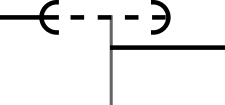
\includegraphics[scale=0.6]{images/souple.png}
    \subcaption{A time constraint with min and max duration}
\end{minipage}	

\caption{Temporal elements of the model}
\label{fig.cst.timenode}
\end{figure}	

The first required primitive is the one able to depict a duration.

We shall call it a \textit{time constraint}.
The time constraint is not necessarily a fixed duration : to allow for interactiveness, 
we must allow it to represent a range, or span of time. For instance, a time constraint may last between 3 and 5 seconds. The maximum can be infinite, to allow for permanent appliances running in a loop. A constraint contains a clock which can be in master or slave mode.

Then, we introduce a mean to synchronize multiple time constraints : a \textit{time node}. 
This allows multiple time constraints to exist both serially, and in parallel, as can be seen in fig.~\ref{fig.cst.timenode}. 
As a byproduct, this allows a clean, graphical separation of concerns while still allowing the author to position related elements close to each other. % Parler du pb avec la verticalité.

Finally, we can assess than constraints also have a logical role, which is of "saying what's next" : a time node will be triggered only after the previous constraints have finished.
% Problème des contraintes à l'édition / à l'exécution : certains arguent que tout devrait être souple à l'exécution et rien à l'édition; d'autre le contraire. D'ou plusieurs modes d'édition grâce à un CSP.

\section{Logical structure}\label{sec.structured}
After the presentation of the time-flow related primitives, we will introduce the first syntax elements that are related to structured programming.
The first element is the condition. For instance, we would like to say : "this temporal constraint will be played only if a given parameter has reached a value of 5".
Hence, this is something that is at a lower level than classic if-then-else constructs; however we can rebuild them afterwards.

Due to the presence of temporal logic, there are actually two kinds of conditions in i-score : 
\begin{itemize}
	\item The purely logical conditions; they cannot modify the flow of time, only be true or false. What matters is their value when they are being evaluated, which will cause the following constraints to be executed - or not. We call these \textit{time events}; visual depiction is in fig.~\ref{fig.logical.events}.
	\item The time-flow controlling conditions. These have more power : they can trigger the execution of a whole time node when they become true. This is why some time constraint will have a minimum and a maximum : the combined min and max of all constraints ending on a given time node will collapse into its execution interval. This interval can be defined at run time in some cases %(cite).
	We call these \textit{triggers}; visual depiction is in fig.~\ref{fig.logical.trigger}.
\end{itemize}

\begin{figure}[h]
	\centering
	\begin{minipage}[b]{.5\linewidth}
		\centering
		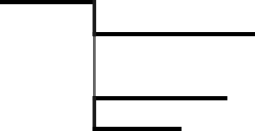
\includegraphics[scale=0.6]{images/events.png}
		\subcaption{Two synchronized events~\\(vertical, bold)}
		\label{fig.logical.events}
	\end{minipage}\begin{minipage}[b]{.5\linewidth}
	\centering
	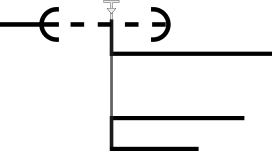
\includegraphics[scale=0.6]{images/trigger.png}
	\subcaption{A trigger (on top)}
	\label{fig.logical.trigger}
    \end{minipage}	

\caption{Logical elements of the model}
\label{fig.logical}
\end{figure}	

Triggers have a lot of influence : once they become true, they will stop all the previous constraints of their time node, evaluate all the time events and start the constraints that follow time events that were true. The default behaviour is that a trigger is also triggered if the maximum duration is reached.

From there, we can start thinking about the implementation of loops. Most people used to audio production software would see loops as the repetition of a simple pattern that lasts a given amount of time. This is in stark contrast with the structured programming loop, where each iteration can yield completely different apparent results.

To allow to do this graphically, we must separate clearly the pattern that the author specified and the result of the execution, which might show this pattern, each time changed a bit, multiple times.

It shall also be noted that when we presented the time nodes and time constraints, we did not mention any explicit restrictions on the nodes that should be before and after a constraint; it can actually be the same. Once the constraint has been read, it triggers the end timenode, which restarts the reading of the constraint. If we put a trigger and minimums \& maximums to our constraint, we can then have loops with iterations of variable durations according to what's occuring on stage.

\begin{figure}
	\centering
	\begin{lstlisting}
	while t < 100
	if a
	[...] short iteration [...]
	else
	[...] long iteration [...]           
	\end{lstlisting}
	\caption{A basic loop}	
	\label{fig.loopcode}
\end{figure}

% TODO ifthenelse
\section{Data structuring}
Now that we have established the entirety of the elements necessary for logical and temporal structuring of scenarios, we shall study how data is handled in the system.
As it could be seen in section~\ref{sec.temporal}, we have two temporal primitives : one that manages durations, and another that manages synchronization.

The kind of data with which i-score is currently the most used is the OSC message, which maps an address in the format "/an/address/here" to a value. Multiple messages together form a state, which is analogous to a cue.

\subsection{Processes}

\begin{figure}[h]
    \centering
    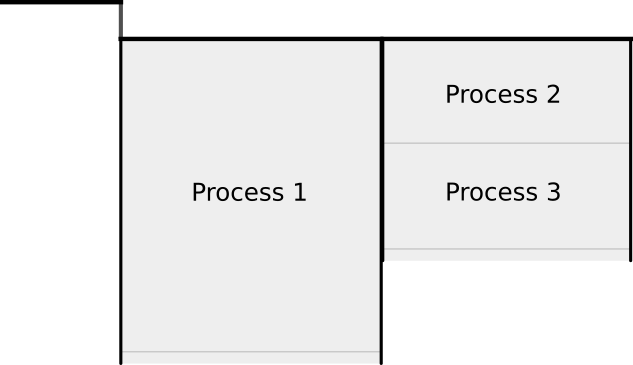
\includegraphics[scale=0.5]{images/processes.png}
    \caption{Processes in constraints}
    \label{fig.processes} 
\end{figure}

To encapsulate data that is meant to last for some amount of time, we build the notion of the process. This is not without similarities with traditional operating system processes, albeit much simpler since they can be made in a purely functional way.

Processes are located in time constraints; a constraint can hold any number of processes. This is shown in fig.~\ref{fig.processes}.

The interface of a process (fig.~\ref{fig.processInterface}) is trivial and allows for a lot of cases common in show-control. The constraint's execution semantics act like a playhead : there is a clock which ticks; on each tick the process's state is pumped. However, it is possible to parametrize what happens with the start and end states which act like parameters to the process. 

Hence, on a purely data-oriented point of view, a process can be seen as a succession of states. However this level of abstraction would be hard to manipulate directly by the authors, especially for automations. We should also note that the state needs not to be known at the moment of writing : one could write a process that returns a random value for each state for instance, or even have processes run their own clock.

By default, a process lasts for as long as its parent constraint. But it is important to keep in mind that since a constraint has a minimal and maximal duration, it would be impossible to have interpolations since you would have to know when the ending has happened to be able to interpolate. 

However, the formalism enables us to have a clean way to give a duration to each process, which will presented in section~\ref{sec.hierarchy}.

\begin{figure}
	\centering
\begin{lstlisting}
    Process:
       State  state(Time)
       State& startState()
       State& endState()
\end{lstlisting}
\caption{Basic interface of a process}
\label{fig.processInterface}
\end{figure}

\subsection{States}
The process have a meaning with regard to durations. However, another common necessity is sending cues at a precise time. For instance, while the position of a lightspot should be interpolated during a few hundred milliseconds to prevent breakage, stopping a music player should be a single message.

In order to achieve this, i-score materializes the notion of instantaneous \textit{state} in a graphical syntax element.

The states are located at the beginning and the end of each temporal constraint. This allows the creation of interpolations between two parameters very easily, by taking a snapshot of a first state, modifying the remote value on the actual device to get a visual feedback and snapshotting again. 

Since states are at both extremities of a time constraint, they happen on a time node. As we saw earlier, a time node represents an instantaneous point in time. 
There are two point of views with regards to the handling of instantaneous data in the system.

\begin{itemize}
	\item The first is that the flow of time is a continuum; an instant does not have a real existence and it can only be approached like an irrational number would be.
	This allows simple temporal reasoning : the author can without a doubt say "B follows A" (in the Allen meaning) and know what the state will be at the intersection of both.
	\item The second is that sometimes, a raw, low-level access to the data that will be scheduled is necessary in order to facilitate work. For instance, in audio software, sometimes sample access is required.   
\end{itemize}
As for audio data, it is sometimes necessary to have a precise access to the behaviour that will take place when there are conflictual data for the same instant. % Note : différent de l'audio car là on a une notion d'unicité avec les timenodes)

This case happens with curves. For instance, if we have two constraints following each other, with curves on the same parameter, we are tempted to say that since the time node represents an instant in time, there should be no difference between the end of the first curve and the beginning of the second. However, sometimes it is practical to have two curves following each other but not at the same value; for instance, this would happen with loops. Since we loop around a single time node, as per section~\ref{sec.structured}, this would enforce having the beginning of the curve equal to the end of the curve, which would not be really practical.

Hence, the user has to specify what value he actually wants to be sent when there is a manifest discrepancy between a logical instant in the scenario, and a physical instant, whose granularity is its of the scheduler, be it the sound card's clock or the network message's clock.

The different possibilities would be keeping a single value, having some behaviour that would involve taking the mean of all the values, or sending each value one after the other.

In order to achieve this, the state is going to save multiple values : 
\begin{itemize}
	\item The values that the user has entered manually.
	\item The values of the previous processes.
	\item The values of the following processes.
\end{itemize}

These values can then be priorized and merged according to arbitrary rules. The user is then able to choose which values are to be synchronized and which ones should be considered independent.
It is also possible to set a filter on the repetition of a given message. For instance, if should happen that a message "/play" was sent to a video player twice in a few milliseconds, the second message could be ignored. This is however done at the adress level, not at the scenario level. The effect can be seen on figure \ref{fig.curvesync}. % Mettre ailleurs

\begin{figure}[h]
	\centering
	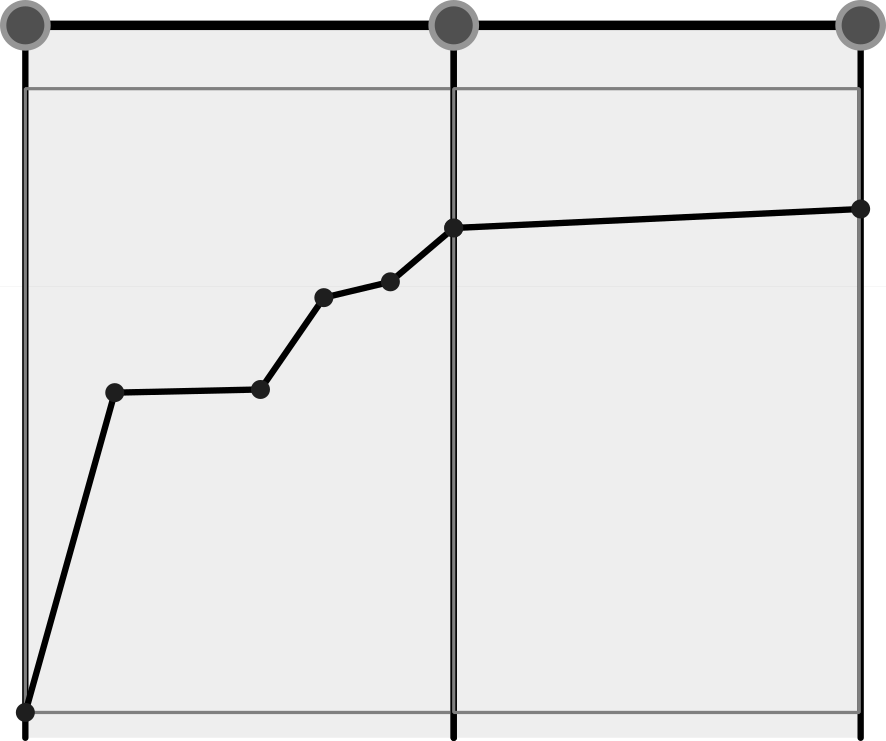
\includegraphics[scale=0.2]{images/curvesync.png}
	\caption{Curves being synchronized on a state. When the user moves either side of the state, the other side will move accordingly}
	\label{fig.curvesync}
\end{figure}

However, not all process shall change value. For instance, somebody could provide a "constant" process that always sends back the same state. Hence, there is actually a request-answer mechanism : when the user inputs a value, either by a process in the other side of the state, or directly in a text field, the other processes are queried and return their new state following this message.

We then have an overview of all of our graphical elements. These make up what we name a \textit{scenario}. By joining together time nodes, time constraints, time events, states, and triggers we can build arbitrarily complex scores. 


% Note : cas ou on a une synchronisation mais la contrainte parente se termine avant

\subsection{Hierarchy}\label{sec.hierarchy}
Thanks to the notion of process, we can introduce the concept of hierarchy. The notion of scenario that we have presented earlier can itself be put into a process. Its specificity is the presence of a starting time node; the scenario is then a tree of constraints that flourishes from it. Practically speaking, all of the interaction with scenarios is done in a scenario process.

The state of the scenario is simple : at a given time, fetch the state of all the running constraints inside of the scenario. This may in turn run triggers, starting the following constraints in the hierarchical scenario. This way, we can have infinite hierarchy.
Furthermore the idea of scenario as a process is interesting for authors because they provide a structured and well-defined unit which can be copy-pasted or saved in a library and reused in other shows.

A side note is the question of the root of a document : if the scenario is purely hierarchic, what is actually present when a document is opened ? There are two possible choices : 
\begin{itemize}
    \item Have the document be contained in a scenario process.
    \item Have the document be contained in a constraint that would itself contain a process. 
\end{itemize}
    
We made the second choice : this way, we can put a trigger on the beginning of the constraint, which would answer to messages like \texttt{/play}. This makes i-score remote-control friendly, in its own formalism.
We can also easily control the play speed of the whole document by adjusting the clock of the constraint.
    
In the same way, the loop is implemented as a process so that it can be manipulated more easily and provide specific GUI rendering, since we do not want to see a constraint wrap around itself, but rather have it repeat its pattern.

Now that we have a loop and a scenario process, we can allow processes in the user interface to get their own duration : this is simply done by embedding them in a scenario process, with a constraint of the given duration at the API level. We can replace the scenario process by a loop process if we want to loop the content of the process for all the duration of the parent constraint instead.

\section{Device trees}
The messages in the states do refer to remote devices : other OSC-compliant software like Max/MSP or PureData instances, or MIDI devices. 

The access inside i-score is done via a common interface, organized as a tree, since it's the most common and familiar way to present a document-like software to the outside. This is commonly refered as object models, the most famous being the HTML Document Object Model. However, there are a lot of other possibilities : Max/MSP and PureData patches can have a hierarchical object model thanks to the Jamoma frameworks presented earlier. Qt software generally revolves around a tree-like object model, too; a more thorough altough older list of such models is given by Richard Adler in \cite{adler1995emerging}.  

This interface in i-score can be reimplemented for other protocols to enable access from i-score to other software. For instance, it could be interesting to have remote procedure call capabilities, via the ways of d-bus, COM+, or other common object-oriented inter-process communication protocols. More easily, it also allows to quickly add discoverable trees of parameters to media software by the ways of the Minuit~\cite{baltazar2009virage}
protocol. 

This have been done for Pure Data, Max/MSP (via the Jamoma frameworks\cite{place2006jamoma}), Quartz Composer, and Qt. The Minuit protocol can use UDP transport (via OSC messages) or TCP transport over websockets. The OSCQuery~\cite{oscquery} 
protocol is also being currently implemented behind this interface. However, we have to keep in mind that not all protocols are born equal : for instance, the MIDI parameter tree is fixed by the MIDI standard and works with a handful of data types. Some software will offer fixed trees of parameters, and some other will offer a much greater flexibility. Likewise, some software would be able to be queried because a query protocol has been directly implemented, while some other, sometimes legacy software or even hardware come with a fixed address space that cannot be queried dynamically. We can prepare such address spaces in a configuration file and load them afterwards.

Generally, parameters have a raw data role, like the volume of a media player. However one can bind any code he wants to a specific address. Hence, some parameters, when triggered, could have the effect of changing the tree structure itself. For instance, one could have a parameter controlling the number of bands in an equalizer. When the number of bands is changed, new addresses allowing to change the gain and frequency of the newly created bands have to be added to the tree.

The parameters in our device tree are currently accessible from the whole software and make for a global state, which is the easiest case. However, we would like to evolve towards the notion of local scope. This notion could be embodied into a process. For instance, a process would be able to control only a subset of the entirety of the addresses : light-related addresses if it's a hierarchical scenario geared towards the control of light and sound-related else.  

This would be our last step towards structured programming since we currently lack structuration of the external data we are accessing. Another question is what to do with addresses that are requested in a scenario but not part of the device tree. A possibility would be to allocate them in a reserved space in the tree (or in the local scope of the process, if available). This would allow us to reach closer towards turing-completeness of our formalism since we would have both loops and a sort of memory allocation - we would mostly lack a way to run actual numeric computations.


\subsection{Local tree}
The document exports its own parameter tree, accessible from the inside and from the outside.
For instance, a scenario will export the triggers that it contains so that they can be manually triggered from the outside (with a companion application running in the internet, or on mobile devices).

This also allows to refer to the time that has currently elapsed at run-time, in order to re-use it in other constraints : for instance, if the first constraint has not been triggered in five seconds, a condition shall become false.

This would also allow to have loops whose duration depends on itself, to have some kind of converging behaviour.

A loopback device is implemented to have fast access to local messages.

Finally, because we can export this local tree over the protocols implemented with our API, this also allows to have remote interfaces, to have a graphical feedback in a web page using WebSockets for instance.

\subsection{Data types in States}
The first goal is to manage classical OSC data types : integers, floating point numbers, strings, arrays...

Apart from this, we also provide two specific data types that are related to the temporal nature of our scenarios.

The first is a "recopy" operator, written \texttt{=}. It is an authoring help and has meaning only in a state at the end of a constraint. It means : "if there is a message with this address at the beginning of a constraint, then take its value".

The second is a "query" operator, written \texttt{?}. The query operator means that the value is to be from another address at run-time. It is then a very basic form of mapping, since the address of the message will take the new value.

This allows to make a state from events depending on what's happening on stage, in order to have mappings. For instance, one could map the audio volume to the position of a dancer on stage at a given time.

However the question of the representation of an unknown value, especially in a curve, is still open. For instance, we could represent it at each frame with its current value; this could mean that a lot of curves could be changing all the time in the scenario while editing, which could be offputting for the authors since they could look elsewhere for a few seconds, and ending not recognizing their scenario because all the curves changed. 


\section{Data-oriented processes}
Now that all of the temporal, structural and data-oriented primitives have been presented, we will show the processes that can be implemented in order to handle sepcific behaviours, like interpolations, for the authors.

We will first study the specific case of the automation, very common in multimedia software, then study one-dimensional and spatial mappings.

\subsection{Automations}
The most important element in a sequencer is the automation : it's the primitive that maps data to time. However, in term of user input mechanism a lot is possible, from traditional WIMP interaction\cite{cohen1999interface} to 3D manipulation of a hardware device mimicking a curve\cite{grossman2003interface}. The two input mechanisms for curves currently implemented in i-score are manual positioning of points and segments, and recording of external values. 

There are two acceptable strategies for recording : the first would be recording the value of a parameter every few milliseconds, which is similar to audio recording. The other would be to record each time a message is received. Since there could be very fast changes of values, we chose to use the second method.
However, since a lot of data can then be received when recording, we use the PSIMPL\cite{psimpl} algorithm library to reduce the number of values after recording to an acceptable range.

i-score provides several facilities for automating data, most notably : 
\begin{itemize}
    \item Discontinuous curves.
    \item Plug-in interface for segments kind.
    \item Multiple edition modes : when moving a point, remove the overlapping points or ignore them.
    \item Locking between points.
\end{itemize}

Currently, the plug-in interface implements linear and exponential segments as they are the most common in multimedia software; we would like to implement other curve families like Béziers curves, sines, and the traditional easing functions\cite{hudson1993animation}.

We would also like to provide pointwise automations, which would be useful for non-numeric data. For instance, this would allow to record the typing of somebody and replay it afterwards.

Finally, an interesting addition would be to use the two special values that we defined earlier, \texttt{?} and \texttt{=}, to specify points that would not only be at the beginning and the end of the automation, but anywhere at the beginning of a segment. \texttt{?} wouldn't work at the end of a segment because we won't know its value until its querying time has arrived. This way, automations could be easily changed dynamically.

\subsection{One-dimensional mappings}
Mappings are a generalization of automations. While automations map time to a given parameter, mappings map, as their name implies, a parameter to another parameter with a transfer function. Since time is an accessible parameter, it is possible to recreate the automation process with the mapping process.

To have a generalized, we can use the query operator, \texttt{?} as the data source instead of the time. It will be queried at each tick by the clock, ask for the current value of the remote parameter, and map it with the transfer function to the output address.

For instance, given the scenarisation abilities presented earlier, one could map the position on the vertical axis of a dancer on stage to the blue color intensity of a spotlight for five seconds, have an automation increasing the red color intensity for  two seconds, and then have another mapping where the dancer controls the red intensity very easily.

A perspective would be the mapping of multi-dimensional parameters in a single view : for instance, what if we want to map the two-dimensional position $[x, y]$ of the dancer, to the $[hue, saturation]$ parameters of the light ?

\subsection{Spatial mappings}
Finally, we will try to present the most generalized form of mappings that is being implemented : spatial mappings. Here, we use the word spatial to refer to parameter spaces which can possibly be mapped into a graphical space that can be manipulated and displayed. 

With automations and one-dimensional mappings, the author has to define a curve that specifies the mapping of a set of data to another set of data.

The idea presented here is a way to allow composers and authors to define such mappings, first directly from mathematical formulas, and then by combining mappings togethers.

Let's give some examples, given two dancers on stage and a spotlight : 
\begin{itemize}
	\item The simplest case would be to power the spotlight when a danser is in an area on stage, like a circle of radius $r$ and center $C$.
	\item We could add some logic : only power the spotlight when both dansers are in the area.
	\item We could also create some data from the data we currently possess : for instance, powering the spotlight when the barycenter (let's name it $G$) of the system composed of both dansers is in the area.
	\item A refinement would be to map the intensity of the light to the distance of $G$ to $C$.
	\item What if $r$ changed ? For instance, the radius of the circle could be mapped to another control : the system would become entirely dynamic.
\end{itemize}

To achieve this kind of flexibility, we define the notion of area. Let's consider $P_1, ... P_N$, $N$ metrical spaces that are related to numerical parameters, and $P = \prod\limits^N_{i=1}P_i$ the product of such spaces. We consider a subset $S$ of $P$ and $1_S$ its characteristic function. 

We can set in advance some parameters to given numerical values : let $\mathbb{X}^N$ be the restriction of $P$ in this case. We call an \textit{area} the restriction of $1_S$ to $\mathbb{X}^N$. Practically speaking, this allows to have areas with some degrees of freedom and some parameters that are set by the user.

For instance, if we take a circle's parametric equation : $(x - a)^2 + (y - b)^2 = c^2$, most of the time we take $x, y$ as variables and $a, b, c$ as parameters. However, we could actually choose the parameters we want to use the result afterwards in computations. For instance, the same equation mapped to a three-dimensional space of variables $x, y, c$ would yield a double cone instead of a circle.

The remaining parameters could be mapped to constants, or parameters taken from the device tree with the query operator to introduce interactive areas.

Then, we can apply computations involving multiple areas like finding intersections, etc. and use the result of such computations to feed either outbound parameters, or the computation of other areas. This allows for a large number of spatial possibilities. An implementation has been started as a process in i-score, using a computer algebra system, GiNaC\cite{bauer2002introduction}, to solve parametric equations with a given parameter set; the biggest open problem is the calculatory complexity for large domains, like areas defined in dimensions greater than 3. However, thanks to the type system of C++ we can seamlessly offer faster paths and approximate solutions for particular known and common shapes, like circles.

\subsection{Extensibility}
Since the process interface is open, anybody can write a process plug-in and be able to use it in i-score to perform his computations in time. For instance, suggested ideas have been to implement a small embedded scripting language, like LUA, as a process, which would allow authors knowledgeable in textual programming to extend the scenarios freely.

There is also a lot of freedom in term of implementation : instead of the current data-pulling model, where a clock recursively checks for all the underlying data and then applies it, we could have a "push" model, where each process has the task of sending its own data. This would work better in many-core environments since processes don't have sharing and locking problem between them, they just send data.

To achieve this, it could be interesting to see how the primitives of a real operating system's scheduler could be used to have a multimedia execution operating system implemented on top of the OS's native processes and inter-process communication like D-Bus.

\section{Tooling}
There are plenty of parts that requires new ideas to be solved in i-score, especially in the area of debugging. Nowadays, many programming language offer very robust tooling, as can be seen in the performance tools that are provided in integrated development environments such as Xcode, Visual Studio, and the various Unix development tool ecosystem\cite{spinellis2014software}. Such tooling can decrease the development time a lot; this should be an aim for the development of artistic interfaces, too.

This is especially important given that a failure in show control can generally cost a lot of money, if used for expositions for instances.

Hence, in the following section, we present the possibilities that are available for visualisation and debugging the execution of scenarios.


\subsection{Debugging}
Debugging is generally used to understand and find out easily why did not a program produce the expected result. Here, we don't have too many problems due to low-level memory management and there cannot be crashes of the interpreter (minus potential bugs in its implementation).  However, as soon as the show's logic becomes complex, it is useful to have tools that makes the authors able to pinpoint where the execution of the show does not match the expected behaviour.

\paragraph{Time Scrub}
The first tool is the time scrub : it allows the displacement in time and the execution of elements in the middle of a scenario process. 

This causes a major problem as soon as there is indeterminism in the score : what should happen if there are two exclusive conditions for instance, and we want to play from the middle of both ? Such problems do not exist in purely linear tools, and authors generally have the habit to scrub wherever they want because of this.

There are multiple possibilities : 

\begin{itemize}
    \item One could define default paths in the tree defined in the process. These paths contain the boolean value for the conditions that are before the time chosen with the scrub, so that the current state can be inferred. However this would take a lot of time on a complex scenario.
    Another possibility would be to have the defaults to false for everything, and require the author to set them manually to true before executing; this would be a hassle most of the time.
    \item It would also be possible to ignore the whole past and only read from the current constraint. However, this causes the same problem than running an arbitrary piece of C code from the middle of it : what happens if the current instructions depend on a previous state being set correctly ?
\end{itemize}

The second problem can be explicited with the following case : if we want to debug a show which involves a smoke machine, it is important to know that they generally require a few tens of seconds of heating before being able to produce smoke. So, in the scenario, the author will certainly have a time constraint that lasts ten seconds before starting to send the smoke generation command. In some cases, not having the pre-heating may break the smoke machine.

However, if we allow the debugging to start from the middle of any constraint, we might if we are not careful trigger the smoke without the heating. It is then necessary to find a way to specify absolute constraints, that are not only present during the execution of the program, but also during the debugging. This would maybe be possible by defining the i-score editing user interface within itself, but requires a lot of manpower. Another possibility would be to have scripting capabilities for the debugging; for instance the Python scripting interfaces of GDB are used for data-flow debugging in~\cite{pouget2013interactive}.

\paragraph{Execution visualization}
Another problem is the visualization of the flow of time once it's running. It is very important to have visual cues of the execution of the program, since not everything may be visible to the spectators, or even in the case of remote monitoring.

Simply showing a time bar like it is done in other sequencers cannot be done here, also because of indeterminism.
For instance, as soon as we have two triggers there will certainly be constraints that used to be synchronized graphically during authoring, but are not occuring at the same time anymore.

The basic possibility would be to simply show time bars per constraints. This may however overwhelm the person keeping an eye on the correct execution if there are too many constraints since there would be a lot of moving elements in the whole screen. This solution is currently implemented.

We also have a problem for infinite constraints : how should they be depicted during execution ? To solve this, we propose to displace and elongate the elements of the scenario according to their position in time. This would then allow to have an unified time bar like in other, linear tools. However, 
this is not without problems either since a lot of graphical elements are now moving at the same time. We also have to save the editing state so that the composer can comes back to it afterwards.

\paragraph{Execution traces}
Finally, it can be useful to save execution traces after the performance. For instance, if something was wrong on stage during a rehearsal, the state of everything up to a few seconds before the bad part should be restored so that it can be practiced without loosing time.
Another interesting use case would be the recording of a performance for automatic, non-interactive replaying; it would be similar to the "rendering" feature of audio workstations.

Traces can come in two formats : the first would be a raw dump of the messages that were sent and received.
The second would be a save of the graphical state if we apply the "moving constraints" solution to the visualization problem.

An interesting problem with traces is the synchronization with the original document. For instance, if a duration is changed in the main document, it could be interesting to keep it up to date in a given execution trace, to retroactively modify what happened if there was only a small deviation from the expected behaviour.

\section{Conclusion}
We presented in this paper an overview of the field of programming and development tools for the authoring of interactive artistic installations, and our contribution in the form of i-score, which is a GUI software, backed by formal semantics and specifications. 

The model of i-score is born of the necessity of fitting programming temporal and structural logic as well as data in a same user interface. For this, we introduce elements based on a syntax which is principally defined graphically, although it can be used from a C++ API.

We argue that using i-score allows the development of artistic installations to be greatly reduced, especially if they involve at the same time a certain degree of structural logic, that has to be encapsulated in time.

We also provide a default set of elements that allows to work with the types of data that the authors are mostly used to : automations and mappings, and we propose ways to extend our model towards complete spatial mappings and a complete calculability model, adapted to time.

Finally, due to the openness of the software and the presence of simple plug-in interfaces, we hope to allow the development of more involved control methods which may require intelligence on the behalf of the authoring software
.
\section{Acknowledgements}
Redacted

\bibliographystyle{SIGCHI-Reference-Format}
\bibliography{base}

\end{document}
